\documentclass[8pt]{article}
\usepackage[UTF8]{ctex}
\usepackage[a4paper]{geometry}

\usepackage{amsthm,amsmath,amssymb}
\usepackage{graphicx}
\usepackage{subfigure}
\usepackage{amsmath}
\usepackage{tabularx}
\usepackage{color}
\usepackage{hyperref}
\usepackage{ulem}
\usepackage{multirow}
\usepackage[cache=false]{minted}
\hypersetup{
	colorlinks=true,
	linkcolor=blue
}

\usepackage{appendix}
\geometry{a4paper,centering,scale=0.8}
\geometry{left=2.0cm, right=2.0cm, top=2.5cm, bottom=2.5cm}
\usepackage[format=hang,font=small,textfont=it]{caption}
\usepackage[nottoc]{tocbibind}

\usepackage{algorithm}
\usepackage{algorithmicx}
\usepackage{algpseudocode}
\usepackage{amssymb}
\usepackage{extarrows}
\usepackage{qcircuit}
\usepackage{fancyhdr}
\usepackage{cleveref}


\usepackage{tikz}  
\usetikzlibrary{arrows.meta}%画箭头用的包

\makeatletter
\def\@maketitle{%
	\newpage
	\begin{center}%
		\let \footnote \thanks
		{\LARGE \@title \par}%
		\vskip 1.5em%
		{\large
			\lineskip .5em%
			\begin{tabular}[t]{c}%
				\@author
			\end{tabular}\par}%
		\vskip 1em%
		{\large \@date}%
	\end{center}%
	\par
	\vskip 1.5em}
\makeatother

\newtheoremstyle{compact}%
{3pt}{3pt}%
{}{}%
{\bfseries}{\textcolor{red}{.}}%  % Note that final punctuation is omitted.
{.5em}{\mbox{\textcolor{red}{\thmname{#1}\thmnumber{ #2}}\thmnote{ (\textcolor{blue}{#3})}}}
\theoremstyle{compact}
\newtheorem{innercustomgeneric}{\customgenericname}
\providecommand{\customgenericname}{}
\newcommand{\newcustomtheorem}[2]{%
	\newenvironment{#1}[1]
	{%
		\renewcommand\customgenericname{#2}%
		\renewcommand\theinnercustomgeneric{##1}%
		\innercustomgeneric
	}
	{\endinnercustomgeneric}
}

\DeclareMathOperator{\card}{card}

\newtheorem{theorem}{定理}
\newtheorem{lemma}{引理}
\newtheorem{definition}{定义}
\newtheorem{proposition}{命题}
\newtheorem{corollary}{推论}
\newtheorem{example}{例}
\newtheorem{claim}{声明}
\newtheorem{remark}{注}
\newtheorem{thesis}{论点}
\newtheorem{Proof}{证明}

\def\obj#1{\textbf{\uline{#1}}}
\def\num#1{\textnormal{\textbf{\mbox{\textcolor{blue}{(#1)}}}}}
\def\le{\leqslant}
\def\ge{\geqslant}
\def\im{\text{im }}
\def\Pr#1{\text{Pr}\left[{#1}\right]}
\def\E#1{\mathbb{E}\left[{#1}\right]}
\def\Var#1{\text{Var}\left[{#1}\right]}

\def\DTIME{\textbf{DTIME}}
\def\NTIME{\textbf{NTIME}}
\def\P{\textbf{P}}
\def\NP{\textbf{NP}}
\def\EXP{\textbf{EXP}}
\def\SPACE{\textbf{SPACE}}
\def\NSPACE{\textbf{NSPACE}}
\def\PSPACE{\textbf{PSPACE}}
\def\NPSPACE{\textbf{NPSPACE}}
\def\L{\textbf{L}}
\def\NL{\textbf{NL}}


\title{\heiti\zihao{1} 计算理论导论\ 课程讲义}
\author{\kaishu\zihao{-3} 周书予\\2000013060@stu.pku.edu.cn}

\CTEXoptions[today=old]
\date{\today}

\begin{document}
\pagestyle{fancy}
\lhead{Introduction to the Theory of Computation}
\rhead{计算理论导论\ 课程笔记}
\chead{2022 Spring}


\crefname{theorem}{定理}{定理}
\crefname{lemma}{引理}{引理}
\crefname{proposition}{命题}{命题}
\crefname{figure}{图}{图}
\crefname{table}{表}{表}	
\maketitle

\section{Outline}
	\begin{enumerate}	
		\item DFA/NFA, Regular Language, Pumping Lemma
		\item Context-free language, Pumping Lemma
		\item Turing Machine
		\item Undecidable Language
		\item Time Complexity \P\ and \NP
		\item Space Complexity \PSPACE, \L\ and \NL
		\item Polynomial Hierarchy
		\item Circuit Complexity
		\item Random Computation
		\item Interactive Proof
		\item (optional) Crypt, Quant, Learning
	\end{enumerate}



\newpage
\section{正则语言}
\begin{definition}[Deterministic Finite Automaton, DFA]
	(确定性)有限自动机是一个五元组$(Q, \Sigma, \delta, q_0, F)$, 其中
	\begin{itemize}
		\item $Q$是称为\obj{状态}的有限集. 
		\item $\Sigma$是称为\obj{字符集}的有限集. 
		\item $\delta: Q \times \Sigma \to Q$被称为\obj{转移函数}. 
		\item $q_0 \in Q$称为\obj{起始态}. 
		\item $F \subseteq Q$称为\obj{接受态(终止态)集合}. 
	\end{itemize}

	称字符串$w = w_1w_2\cdots w_m(w_i \in \Sigma)$可以被DFA $M = (Q, \Sigma, \delta, q_0, F)$接受, 如果存在状态序列$r_0, r_1, \cdots, r_m \in Q$满足\num{i}$r_0 = q_0$, \num{ii}$r_{i+1} = \delta(r_i, w_{i+1}) \ (\forall i = 0, 1, \cdots, m-1)$, \num{iii}$r_m \in F$. 

	所有可被$M$识别的字符串$w$构成集合$A$, 则称$A$是 DFA $M$的语言(或者说 DFA $M$识别/接受$A$), 记为$L(M) = A$.
\end{definition}
\begin{definition}[正则语言]
	正则语言就是能够被有限自动机识别的语言. 
\end{definition}
\begin{definition}[正则操作]
	定义如下三种正则操作
	\begin{itemize}
		\item \obj{Union}: $A \cup B = \{x | x \in A \textrm{ or } x \in B\}$.
		\item \obj{Concatenation}: $A \circ B = \{xy | x \in A \textrm{ and } y \in B\}$.
		\item \obj{Star}: $A^* = \{x_1x_2\cdots x_k | k \ge 0 \textrm{ and each } x_i \in A\}$.
	\end{itemize}
\end{definition}
\begin{remark}
	补集$\overline{A} = \Sigma^* - A$操作在正则语言下是封闭的: 只需要把终止态集合$F$改成$Q - F$即可.
\end{remark}
\begin{theorem}
	正则操作 union 在正则语言下是封闭的: 把两个自动机放在一起跑就行了. 
\end{theorem}
由于只利用已有的有限自动机模型证明 concatenation 和 star 的封闭性是困难的, 我们引入“非确定性”. 
\begin{definition}[Nondeterministic Finite Automaton, NFA]
	非确定性有限自动机是一个五元组$(Q, \Sigma, \delta, q_0, F)$, 其中$\delta$不再是$Q \times \Sigma \to Q$的函数, 而是$Q \times \Sigma_{\varepsilon} \to \mathcal P(Q)$的, 其中$\mathcal P$表示幂集, $\Sigma_{\varepsilon}$表示$\Sigma \cup \{\varepsilon\}$. 

	相应的, 称字符串$w = w_1w_2\cdots w_m(w_i \in \Sigma)$可以被NFA $N = (Q, \Sigma, \delta, q_0, F)$接受, 如果$w$可以写成$w = y_1y_2\cdots y_{m'}(y_i \in \Sigma_{\varepsilon})$, 且存在状态序列$r_0, r_1, \cdots, r_{m'} \in Q$满足\num{i}$r_0 = q_0$, \num{ii}$r_{i+1} \in \delta(r_i, y_{i+1})$\ $(\forall i = 0, 1, \cdots, {m'}-1)$, \num{iii}$r_{m'} \in F$. 
\end{definition}
\begin{remark}
	DFA的每个状态对每种字符都有恰好一条转移出边, 而相对的, NFA可能有零条、一条或者多条, 有几条出边就表示会创建出多少个独立的“后继进程”. 此外还存在$\varepsilon$的出边, 表示可以不输入任何字符创建进程. 
\end{remark}
\begin{theorem}[NFA与DFA的等价性]
	任何NFA都存在等效的DFA. 
\end{theorem}
\begin{proof}
	对$k$个状态的NFA, 构造一个$2^k$个状态的DFA, 每个状态表示“可能处在的NFA状态”的子集. 

	形式化的, 对于 NFA $M = (Q, \Sigma, \delta, q_0, F)$, 构造 DFA $M' = (Q', \Sigma, \delta', q_0', F')$, 其中
	\begin{itemize}
		\item $Q' = \mathcal P(Q)$.
		\item $\forall R \in Q', a \in \Sigma, \delta'(R, a) = \bigcup_{r \in R}\delta(r, a)$.
		\item $q_0' = \{q_0\}$.
		\item $F' = \{R \in Q' | R \cap F \neq \varnothing\}$.
	\end{itemize}
\end{proof}
\begin{corollary}
	一个语言是正则的当且仅当可以被一台非确定性有限自动机识别. 
\end{corollary}
\begin{theorem}
	union, concatenation 和 star 在正则语言下都是封闭的. 
\end{theorem}
\begin{proof}
	不多说了看图. 

	\begin{figure}[htbp]
		\centering
		\subfigure[proof for union]{
			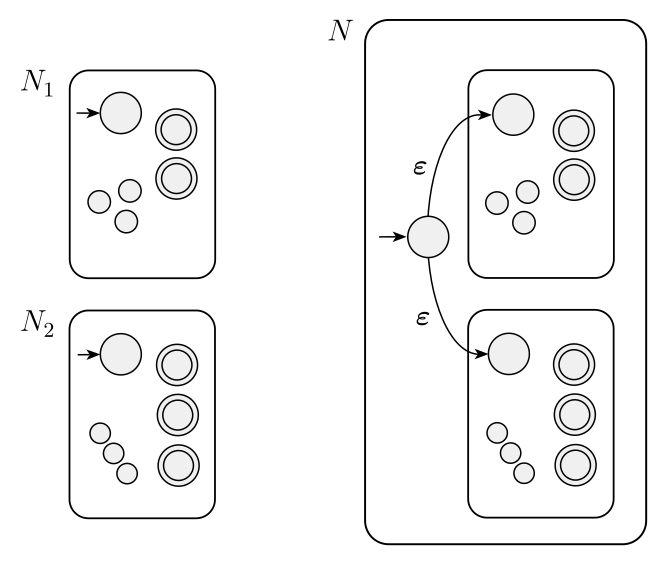
\includegraphics[scale=0.25]{pic/union.png}
		}
		\quad
		\subfigure[proof for concatenation]{
			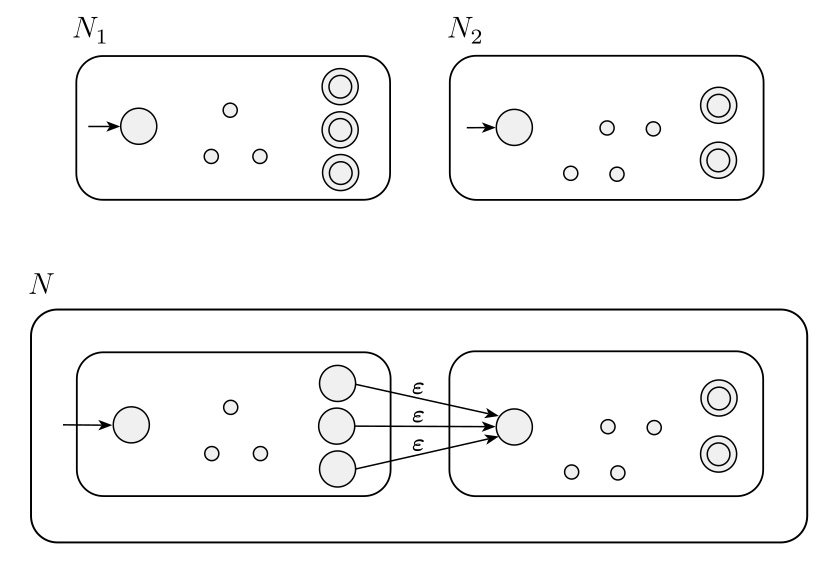
\includegraphics[scale=0.25]{pic/concat.png}
		}
		\quad
			\subfigure[proof for star]{
			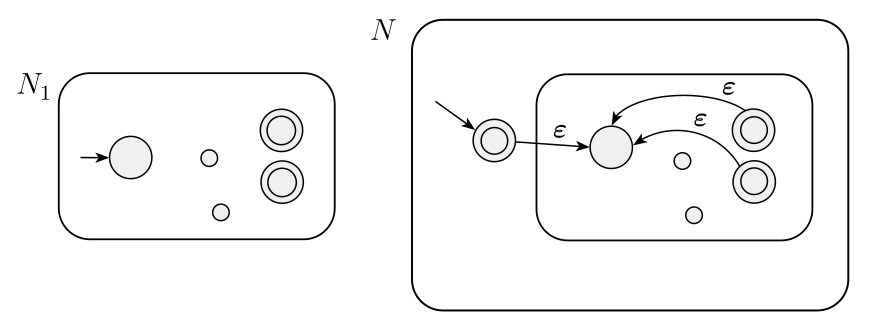
\includegraphics[scale=0.25]{pic/star.png}
		}
	\end{figure}
\end{proof}
\begin{definition}[正则表达式]
	称$R$是正则表达式, 如果$R$为
	\begin{itemize}
		\item $\{a\}$, 其中$a$是字符集$\Sigma$中的某个元素
		\item $\{\varepsilon\}$, 其中$\varepsilon$表示空串
		\item $\varnothing$
		\item $(R_1 \cup R_2)$, 其中$R_1, R_2$是某两个正则表达式
		\item $(R_1 \circ R_2)$, 其中$R_1, R_2$是某两个正则表达式
		\item $(R_1^*)$, 其中$R_1$是某个正则表达式
	\end{itemize}
\end{definition}
\begin{example}
	对于任意正则表达式$R$, $R \cup \varnothing = R \circ \varepsilon = R$, $R \circ \varnothing = \varnothing$, $\varnothing^* = \{\varepsilon\}$. 
\end{example}
\begin{theorem}[正则表达式与有限自动机的等价性]
	一个语言是正则的当且仅当它可以被一个正则表达式描述. 
\end{theorem}
\begin{proof}
	“$\Leftarrow$”的证明是简单的, 只需要根据正则表达式$R$构造NFA, 利用“union, concatenation, star的封闭性”的构造性证明即可. 

	“$\Rightarrow$”的证明中, 我们引入GNFA的定义(每条转移边上的label是一个正则表达式), 然后分别展示如何把DFA转化成GNFA以及如何根据GNFA构造正则表达式. 

	DFA转GNFA是简单的——只需要额外加入两个状态表示$q_{\text{start}}$和$q_{\text{accept}}$即可. 

	观察到一个GNFA有$k \ge 2$个状态. 如果$k=2$, 那么$q_{\text{start}}$到$q_{\text{accept}}$的转移边上的正则表达式就是该有限自动机对应的正则表达式. 如果$k > 2$, 那么考虑选出一个状态$q_{\text{rip}}$删除, 此时对于$q_i, q_j \in Q \setminus \{q_{\text{rip}}\}$, 如果$\delta(q_i,  q_{\text{rip}}) = R_1, \delta(q_{\text{rip}}, q_{\text{rip}}) = R_2, \delta(q_{\text{rip}}, q_j) = R_3, \delta(q_i, q_j) = R_4$, 则修改$\delta'(q_i, q_j) = (R_1)(R_2)^*(R_3) \cup (R_4)$. 归纳即可. 
\end{proof}
\begin{definition}[Generalized Nondeterministic Finite Automaton, GNFA]
	广义非确定性有限自动机是一个五元组$(Q, \Sigma, \delta, q_{\text{start}}, q_{\text{accept}})$, 其中$\delta$是$(Q \setminus \{q_{\text{accept}}\}) \times (Q \setminus \{q_{\text{start}}\}) \to \mathcal R$的转移函数, $\mathcal R$表示字符集$\Sigma$上的所有正则表达式. 注意不失一般性地要求了只有唯一的接受态, 以及$q_{\text{start}} \neq q_{\text{accept}}$. 
\end{definition}
\begin{theorem}[Pumping Lemma for Regular Language]
	如果$A$是正则语言, 那么存在一个数$p$ (称为\obj{pumping length}), 使得对于任意$A$中长度至少为$p$的字符串$s$, $s$都可分成三部分$s = xyz$满足
	\begin{itemize}
		\item for each $i \ge 0$, $xy^iz \in A$,
		\item $|y| > 0$,
		\item $|xy| \le p$.
	\end{itemize}
\end{theorem}
\begin{proof}
	取 pumping length $p$ 为识别此正则语言的 DFA $M$的状态集大小$|Q|$. 对于任意长度至少为$p$的$s \in A$, 其经过的状态序列至少长为$p+1$. 根据\obj{鸽巢原理}, 存在一个状态$q$经过了至少两次, 于是把从$q_{\text{start}}$走到$q$的部分视作$x$, $q$回到自身的环视作$y$, 从$q$走到$q_{\text{accept}}$的部分视作$z$, 便构造出了划分. 
\end{proof}
\begin{remark}
	利用 pumping lemma 可以证明某个语言$B$不是正则语言, 通用的方式是:先假设$B$是正则的, 导出 pumping length $p$的存在性, 然后根据这个$p$构造$s \in B$, 并验证其\obj{不能}被划分为$s = xyz$. 第三个条件$|xy| \le p$有时也是有用的. 
\end{remark}
\begin{example}
	$B = \{0^n1^n | n \ge 0\}$ 不是正则语言.
\end{example}
\begin{proof}
	假设 $B$ 是正则语言, 那么就存在 pumping length $p$. 考虑串 $0^p1^p$, 无论 $y$ 取其何种子串, $xyyz$ 都不可能 $\in B$. 因此 $B$ 不是正则语言.
\end{proof}
\begin{example}
	$C = \{w | w \text{ has an equal number of 0s and 1s}\}$ 不是正则语言.
\end{example}
\begin{proof}
	假设 $C$ 是正则语言, 那么就存在 pumping length $p$. 考虑串 $0^p1^p$, 注意到我们要求了 $|xy| \le p$, 所以 $y$ 只能包含 $0$, 此时 $xyyz \notin B$. 因此 $C$ 不是正则语言.
	
	\textit{另一种证法是: 考虑 $C \cap 0^*1^* = B$, 正则语言在 intersection 下是封闭的, 所以$C$正则会导出$B$正则.}
\end{proof}
\begin{example}
	$F = \{ww | w \in \{0, 1\}^*\}$ 不是正则语言.
\end{example}
\begin{proof}
	考虑串 $0^p10^p1$, 注意到 $y$ 只能包含 $0$, 从而$xyyz \notin F$, 因此$F$不是正则语言.
\end{proof}

\begin{example}
	$D = \{1^{n^2} | n \ge 0\}$ 不是正则语言.
\end{example}
\begin{proof}
	考虑串 $1^{p^2}$. 由于 $|y| \le p$, 所以 $|xyyz| = p(p+1) < (p+1)^2$ 不可能是完全平方数, $xyyz \notin D$, 说明$D$不是正则语言.
\end{proof}
\begin{example}
	$E = \{0^i1^j | i > j\}$不是正则语言. 
\end{example}
\begin{proof}
	考虑串$0^{p+1}1^p$, $y$只能包含 $0$, 且$|y| > 0$, 因此$xz$中$0$的个数不超过 $1$的个数, $xz \notin E$, 说明 $E$ 不是正则语言.
\end{proof}
\newpage
\section{上下文无关文法}
\begin{definition}[Context-Free Grammar/Language, CFG/CFL]
	一个上下文无关文法是一个四元组$(V, \Sigma, R, S)$, 其中
	\begin{itemize}
		\item $V$是称为\obj{变量}的有限集, 
		\item $\Sigma$是称为\obj{终止符}的有限集, 与$V$不交, 
		\item $R$是称为\obj{规则}的有限集, 是从$V$到$(V \cup \Sigma)^*$的映射, 
		\item $S \in V$称为\obj{起始变量}. 
	\end{itemize}

	上下文无关语言就是上下文无关文法导出的语言, 即$\{w \in \Sigma^* | S \overset{*}{\Rightarrow} w\}$. 
\end{definition}
\begin{proposition}
	CFG 的描述能力严格强于有限自动机(或者正则表达式). 
\end{proposition}
\begin{proof}
	对于任意的DFA, 都可以构造与其等价的CFG:对每个状态$q_i$构造一个变量$R_i$, 起始变量$R_0$对应起始态$q_0$, 如果$\delta(q_i, a) = q_j$, 就添加规则$R_i \to aR_j$, 而如果$q_i$是接受态, 就添加规则$R_i \to \varepsilon$. 

	而显然存在可被 CFG 描述的非正则语言, 比如$\{0^n1^n | n \in \mathbb N\}$. 
\end{proof}
\begin{definition}[歧义性]
	
\end{definition}
\begin{definition}[Chomsky 范式]
	
\end{definition}
\begin{definition}[Pushdown Automata, PDA]
	下推自动机是一个六元组$(Q, \Sigma, \Gamma, \delta, q_0, F)$, 其中
	\begin{itemize}
		\item $Q$是状态集, 
		\item $\Sigma$是输入字符集, 
		\item $\Gamma$是栈字符集, 
		\item $\delta: Q \times \Sigma_{\varepsilon} \times \Gamma_{\varepsilon} \to \mathcal P(Q \times \Gamma_{\varepsilon})$是转移函数, 
		\item $q_0 \in Q$是起始态, 
		\item $F \subseteq Q$是接受态集合. 
	\end{itemize}

	其中$\Sigma_{\varepsilon}, \Gamma_{\varepsilon}$分别表示$\Sigma \cup \{\varepsilon\}, \Gamma \cup \{\varepsilon\}$, 幂集$\mathcal P$暗含了下推自动机是 nondeterministic 的. 

	称字符串$w = w_1w_2\cdots w_m(w_i \in \Sigma_{\varepsilon})$可以被 PDA $M = (Q, \Sigma, \Gamma, \delta, q_0, F)$接受, 如果存在状态序列$r_0, r_1, \cdots, r_m \in Q$和字符串(栈)序列$s_0, s_1, \cdots, s_m \in \Gamma^*$, 满足
	\begin{itemize}
		\item $r_0 = q_0, s_0 = \varepsilon$,
		\item For $i = 0, 1, \cdots, m-1$, $(r_{i+1}, b) \in \delta(r_i, w_{i+1}, a)$, where $s_i = at, s_{i+1}=bt$ for some $a, b \in \Gamma_{\varepsilon}$ and $t \in \Gamma^*$,
		\item $r_m \in F$.
	\end{itemize}
\end{definition}

\begin{theorem}[下推自动机与上下文无关文法的等价性]
	一个语言是上下文无关的, 当且仅当存在某个下推自动机可以识别它. 
\end{theorem}
\begin{proof}
	“$\Rightarrow$”: 需要根据 CFG 来构造 PDA. 一开始把 CFG 的起始变量写在栈上, 利用 nondeterminism 尝试每一种变量的替换方式. 每次只考虑替换栈顶的变量, 而如果栈顶是一个终止符, 就直接和输入匹配掉, 保证栈顶始终是一个尚未替换的变量. 当输入匹配完且栈为空时, 代表输入串可接受. 

	“$\Leftarrow$”: 需要根据 PDA 来构造 CFG. 不妨假设\footnote{需要简短地说明转化的可行性. }该 PDA 有如下特性:\num{i}只有一个接受态$q_{\text{accept}}$, \num{ii}会在接受前清空栈, \num{iii}每次转移都会要么 push 要么 pop, 没有 both 和 neither 的情况. 构造变量$A_{pq}$表示所有能够使 PDA 从“状态$p$且栈空”转移到“状态$q$且栈空”的串组成的语言, 其中$A_{q_0q_{\text{accept}}}$是该 CFG 的起始变量. 按如下方式构造 CFG 的规则集合:
	\begin{itemize}
		\item 对于任意$p, q, r, s \in Q, u \in \Gamma, a, b \in \Sigma_{\varepsilon}$, 如果$(r, u) \in \delta(p, a, \varepsilon), (q, \varepsilon) \in \delta(s, b, u)$, 就添加规则$A_{pq} \to a A_{rs} b$, 
		\item 对于任意$p, q, r \in Q$, 添加规则$A_{pq} \to A_{pr}A_{rq}$, 
		\item 对于任意$p \in Q$, 添加规则$A_{pp} \to \varepsilon$. 
	\end{itemize}

	构造思路来源于考虑压栈弹栈的括号序列, 该序列要么被一个大括号包裹(第一种), 要么由两个括号序列组成(第二种). 可以归纳证明构造方式与含义的等价性. 
\end{proof}
\begin{theorem}[Pumping Lemma for CFL]
	如果$A$是上下文无关语言, 那么存在一个数$p$(称为\obj{pumping length}), 使得对于任意$A$中长度至少为$p$的字符串$s$, $s$都可以分成五部分$s = uvxyz$满足
	\begin{itemize}
		\item for each $i \ge 0, uv^ixy^iz \in A$,
		\item $|vy| > 0$,
		\item $|vxy| \le p$.
	\end{itemize}
\end{theorem}
\begin{proof}
	设$b$为规则中的最大“度数”, 即替换字符串的最大长度. 如果 parse tree 的树高是$h$(不计叶子), 那么生成的字符串长度至多为$b^h$. 

	取 pumping length $p$ 为$b^{|V|+1}$. 一方面, 长度至少为$p$的串对应的 parse tree 树高至少为$|V| + 1$, 即存在一条“直链”上有至少$|V| + 1$个变量, 根据\obj{鸽巢原理}, 存在一个变量出现至少两次, 记为$R$, 那么对于$R$就可以无限复制或者把两次出现压缩成一次(如图). 

	为了满足第三个条件, 取$R$为满足条件的“深度最大”的, 即两个$R$都出现在最底下$|V| + 1$层. 此时$|vxy|$对应第一个$R$的子树大小, 受深度限制不超过$b^{|V| + 1} = p$. 
	\begin{center}
		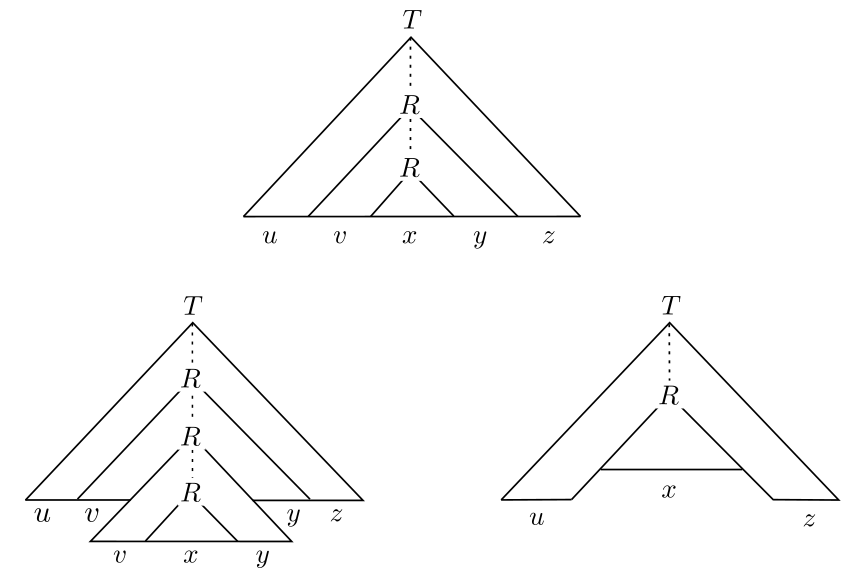
\includegraphics[scale=0.3]{pic/pumping_for_CFL.png}		
	\end{center}
\end{proof}
\begin{example}
	$B = \{a^nb^nc^n | n \ge 0\}, C = \{a^ib^jc^k | 0 \le i \le j \le k\}, D = \{ww | w \in \{0, 1\}^*\}$都不是上下文无关语言. 
\end{example}

\newpage
\section{图灵机}

\begin{definition}[图灵机]
	一台图灵机(Turing Machine, TM)$M$可用三元组$(\Gamma, Q, \delta)$来描述, 其中
	\begin{itemize}
		\item 有限集$\Gamma$为$M$的字符集. 我们认为$\Gamma$中包含$\Box$表示空格, 以及$\triangleright$表示起始标识. 
		\item 有限集$Q$为$M$的状态集. 我们认为$Q$中包含$q_{\text{start}}$表示起始状态, 以及$q_{\text{halt}}$表示停机状态. 
		\item 转移函数$\delta: Q \times \Gamma^{k} \to Q \times \Gamma^{k-1} \times \{L, S, R\}^{k}$, 其中$k \ge 2$为纸带条数. 
	\end{itemize}
	除非特殊说明, 一般认为第一张纸带是\obj{只读}的. 
\end{definition}
\begin{definition}[函数的计算, 运行时间]
	设函数$f: \{0,  1\}^* \to \{0, 1\}^*$以及$T: \mathbb{N} \to \mathbb{N}$, 令$M$为一图灵机. 我们称$M$计算了函数$f$, 如果对于任意$x \in \{0, 1\}^*$, 只要$M$的输入被初始化为$x$, 它就能在输出纸带上写下$f(x)$并停机. 称$M$在$T(n)$的时间内计算了$f$, 如果它计算每个$x$都只需要不超过$T(|x|)$的时间. 
\end{definition}
\begin{definition}[Time constructible functions]
	称一个函数$T: \mathbb N \to \mathbb N$是time constructible的, 如果$T(n) \ge n$且存在运行时间为$T(n)$的计算函数$x \to T(|x|)$的图灵机$M$. 
\end{definition}
\begin{proposition}[大字符集规约到小字符集]
	对于任意$f: \{0, 1\}^* \to \{0, 1\}$以及time constructible的函数$T: \mathbb{N} \to \mathbb{N}$, 如果$f$可以被图灵机$M$以$T(n)$时间计算, 那么它也可以被一台字符集为$\{0, 1, \Box, \triangleright\}$的图灵机$\tilde{M}$以$4\log |\Gamma|T(n)$的时间计算. 
\end{proposition}
\begin{proposition}[多条纸带规约到一条纸袋]
	对于任意$f: \{0, 1\}^* \to \{0, 1\}$以及time constructible的函数$T: \mathbb{N} \to \mathbb{N}$, 如果$f$可以被有$k$条纸带的图灵机$M$以$T(n)$时间计算, 那么它也可以被一台单纸带图灵机$\tilde{M}$以$5kT^2(n)$的时间计算. 单纸带指的是只有一条可读可写的纸带, 它同时扮演了输入、工作和输出纸带的角色. 
\end{proposition}
\begin{remark}[健忘的图灵机, oblivious Turing Machine]
	头部移动与输入长度有关, 而与输入的具体内容无关, 即对于任意$x \in \{0, 1\}^*$以及$i \in \mathbb N$, $M(x)$执行到第$i$步时读写头的位置是只关于$|x|$和$i$的函数. 可以证明图灵机可以平方规约到健忘的图灵机. 
\end{remark}
\begin{proposition}[双向图灵机规约到单向图灵机]
	对于任意$f: \{0, 1\}^* \to \{0, 1\}$以及time constructible的函数$T: \mathbb{N} \to \mathbb{N}$, 如果$f$可以被双向图灵机(纸带的两个方向都有无限长)$M$以$T(n)$时间计算, 那么它也可以被一台单向图灵机$\tilde{M}$以$4T(n)$的时间计算. 
\end{proposition}
\begin{theorem}[通用图灵机存在]
	存在图灵机$\mathcal U$使得对于任意$x, \alpha \in \{0, 1\}^*$, $\mathcal U(x, \alpha) = M_{\alpha}(x)$, 其中$M_{\alpha}$为被$\alpha$表示的图灵机. 进一步地, 如果$M_{\alpha}$对于$x$在$T$步内停机, 则$\mathcal U(x, \alpha)$可以在$CT\log T$步内停机, 其中$C$是一个仅依赖于$M_{\alpha}$的字符集大小、纸袋条数、状态数的常数. 
\end{theorem}
\begin{definition}[\DTIME 与 \P]
	对于函数$T: \mathbb N \to \mathbb N$, 称语言$L \in \DTIME(T(n))$, 如果存在常数$c > 0$和一台运行时间为$c \cdot T(n)$的图灵机可以决定$L$. 

	$\P = \bigcup_{c \ge 1}\DTIME(n^c)$. 
\end{definition}
\begin{thesis}[Church-Turing thesis]
	任何物理上可实现的计算设备都可以被图灵机模拟. 
\end{thesis}

\begin{Proof}[时间复杂度$O(T^2)$的模拟]
	
\end{Proof}
\begin{Proof}[时间复杂度$O(T  \log T)$的模拟]
	
\end{Proof}


\newpage
\section{NP 与 NP-complete}

\begin{definition}[\NP]
	语言$L \subseteq \{0, 1\}^*$属于\NP, 如果存在一个多项式$p: \mathbb N \to \mathbb N$和一个多项式时间图灵机$M$(称其为$L$的\obj{verifier})使得对于任意的$x \in \{0, 1\}^*$, 都有
	$$x \in L \Leftrightarrow \exists u \in \{0, 1\}^{p(|x|)}, M(x, u) = 1$$
	如果$x \in L$与$u \in \{0, 1\}^{p(|x|)}$满足$M(x, u) = 1$, 则称$u$是$x$的一个\obj{certificate}. 
\end{definition}
\begin{proposition}
	定义$\EXP = \bigcup_{c > 1} \DTIME(2^{n^c})$, 则$\P \subseteq \NP \subseteq \EXP$. 
\end{proposition}
\begin{definition}[非确定图灵机与\NTIME]
	非确定图灵机(Nondeterministic Turing Machine, NDTM)是有两个转移函数$\delta_0, \delta_1$和一个特定状态$q_{\text{accept}}$的图灵机$M$, 每步转移时, 可以任意选择遵从某一个转移函数. 对于输入$x$, 称$M(x) = 1$当且仅当存在一个选择序列可以使$M$到达$q_{\text{accept}}$状态, 否则——任意选择序列都无法在停机前到达$q_{\text{accept}}$——就认为$M(x) = 0$. 称$M$的运行时间为$T(n)$, 如果对于任意输入$x \in \{0, 1\}^*$以及任意的选择序列, $M$都会在$T(|x|)$步内到达$q_{\text{accept}}$或者$q_{\text{halt}}$. 

	对于$T: \mathbb N \to \mathbb N$和语言$L \subseteq \{0, 1\}^*$, 称$L \in \NTIME(T(n))$, 如果存在常数$c > 0$和一个运行时间为$c \cdot T(n)$的非确定图灵机$M$, 满足对于任意的$x \in \{0, 1\}^*$, $x \in L \Leftrightarrow M(x) = 1$. 
\end{definition}
\begin{theorem}
	$\NP = \bigcup_{c \ge 1} \NTIME(n^c)$. 
\end{theorem}
\begin{proof}
	证明的核心思路在于非确定图灵机的选择序列可以看作$x$的一个certificate, 反之亦然. 
\end{proof}

\begin{definition}[规约, \NP-hard与\NP-complete]
	称语言$L \subseteq \{0, 1\}^*$可\obj{多项式时间规约}到语言$L' \subseteq \{0, 1\}^*$(记作$L \le_p L'$), 如果存在一个多项式时间可计算函数$f: \{0, 1\}^* \to \{0, 1\}^*$使得对于任意$x \in \{0, 1\}^*$, $x \in L \Leftrightarrow f(x) \in L'$. 

	称$L'$是\NP-hard, 如果对于任意$L \in \NP$, $L \le_p L'$. \NP-complete $=$ \NP\ $\cap$ \NP-hard.  
\end{definition}
\begin{theorem}[$\le_p$的传递性]
	\begin{itemize}
		\item 若$L \le_p L'$且$L' \le_p L''$, 则$L \le_p L''$. 
		\item 如果$L$是\NP-hard且$L \in P$, 则$\P = \NP$. 
		\item 如果$L$是\NP-complete, 则$L \in P$当且仅当$\P = \NP$. 
	\end{itemize}
\end{theorem}
\begin{theorem}[Cook-Levin Theorem]
	$\textsf{SAT}, \textsf{3SAT}$是\NP-complete. 
\end{theorem}

\newpage
\section{对角线法则}
\begin{theorem}[Time Hierarchy Theorem]
	$f, g$是满足$f(n) \log f(n) = o(g(n))$的time constructible的函数, 则
	$$\DTIME(f(n)) \subsetneq \DTIME(g(n))$$
	\label{time_hierarchy_thm}
\end{theorem}
\begin{proof}
	考虑这样的图灵机$D$:对于$x$, 用通用图灵机$\mathcal{U}$模拟$M_x$($x$描述的图灵机)运行至多$g(|x|)$步(是$U$的$g(|x|)$步而不是$M_x$的$g(|x|)$步), 如果$\mathcal{U}$在$g(|x|)$步数内输出了$b \in \{0, 1\}$, 则$D$输出$1-b$;否则$D$输出$0$. 

	根据定义, $D$对于任何输入$x$都会在$g(|x|)$步内停机, 因此$D$决定的语言$L$属于$\DTIME(g(n))$. 我们通过反证法证明$L \notin \DTIME(f(n))$. 先叙述否命题:存在图灵机$M$和常数$c$, 使得对于任意输入$x \in \{0, 1\}^*$, $M$都能在$cf(|x|)$步内输出与$D$相同的结果. 

	对于输入$x$, 用通用图灵机$\mathcal{U}$模拟$M$只需要$c'cf(|x|)\log f(|x|)$步, 其中$c'$是不依赖于$|x|$的一个常数. 由于$f(n) \log f(n) = o(g(n))$\footnote{little-$o$不能替换成big-$O$, 我只能说懂的都懂. }, 故存在充分大的$n_0$使得$g(n) > c'cf(n) \log f(n)$对于任意$n \ge n_0$均成立. 令$x'$表示$M$的某个长度大于$n_0$的表示, 那么
	\begin{itemize}
		\item $D$会输出与$M$相同的结果, 因为这是$M$的定义;
		\item $D$会输出与$M$不同的结果, 因为$c'cf(n)\log f(n) < g(n)$使得$\mathcal U$对$M$的模拟已经结束了, 根据$D$的定义, $D$应该输出相反的结果. 
	\end{itemize}

	产生了矛盾. 因此$\DTIME(f(n)) \subsetneq \DTIME(g(n))$. 
\end{proof}
\begin{theorem}[Nondeterministic Time Hierarchy Theorem]
	$f, g$是满足$f(n + 1) = o(g(n))$的time constructible的函数, 则
	$$\NTIME(f(n)) \subsetneq \NTIME(g(n))$$
\end{theorem}
\begin{theorem}[Ladner's Theorem]
	如果$\P \neq \NP$, 则存在语言$L \in \NP \setminus \P$, 即非 \NP-complete 的 \NP 语言. 
\end{theorem}

\newpage
\section{空间复杂性}
\begin{definition}[运行空间, \SPACE 与 \NSPACE]
	对于$S: \mathbb N \to \mathbb N$和$L \subseteq \{0, 1\}^*$, 称$L \in \SPACE(S(n))$, 如果存在常数$c$以及可以决定$L$的图灵机$M$, 满足在对任意长度为$n$的输入的计算中, $M$只会访问到至多$c \cdot S(n)$个work tapes上(不包含input)的位置, 称$M$的运行空间为$O(S(n))$. 

	类似地可以定义$\NSPACE$, 这里要求在任何一种决策下用到的位置数量都不超过$c \cdot S(n)$. 
\end{definition}
\begin{definition}[Space constructible functions]
	称$S: \mathbb N \to \mathbb N$是space constructible的, 如果存在图灵机可以对于输入$x$, 在$O(S(|x|))$的空间内计算$S(|x|)$. 
\end{definition}
\begin{remark}
	相比于 time constructible functions, 我们不要求 space constructible functions 满足 $S(n) \ge n$, 但为了能够“记住在输入纸带上的位置”, 我们一般会要求 $S(n) \ge \log n$. 
\end{remark}
\begin{theorem}
	对于任何 space constructible 的函数$S: \mathbb N \to \mathbb N$, 有
	$$\DTIME(S(n)) \subseteq \SPACE(S(n)) \subseteq \NSPACE(S(n)) \subseteq \DTIME(2^{O(S(n))})$$
	\label{time_and_space}
\end{theorem}
\begin{proof}
	前两个$\subseteq$都是平凡的, 只考虑证明最后一个. 

	我们称一台(确定或非确定)图灵机$M$的一个\obj{configuration}包含\num{i}work tape上的所有非空字符;\num{ii}所有纸带的head位置;\num{iii}$M$所处的状态, 则对于确定的输入$x \in \{0, 1\}^*$, 一个configuration的后继configuration是\num{a}对于图灵机来说, 唯一确定的;\num{b}对于非确定图灵机来说, 至多唯二确定的. 把configuration之间的转移看成一张有向图, 记作$G_{M, x}$. 不失一般性假设$M$只有一种configuration $C_{\text{accept}}$满足“输出$1$后停机”(可以让图灵机在停机前擦除所有中间记录), 这样$M(x) = 1$就等价于$G_{M, x}$中存在一条$C_{\text{start}}$到$C_{\text{accept}}$的路径. 

	陈述两个事实:
	\begin{itemize}
		\item 给定$M, x$, $G_{M, x}$中的每个节点用$O(S(n))$个bit来表示, 也即, $G_{M, x}$只有$2^{O(S(n))}$个节点. 
		\item 对于任意两个configuration $C, C'$, 存在$O(S(n))$大小的CNF $\varphi_{M, x}$满足$\varphi_{M, x}(C, C') = 1$当且仅当$G_{M, x}$中$C$有边连向$C'$. 
	\end{itemize}

	因此用$2^{O(S(n))}$的时间把整张$G_{M, x}$建出来, 再 BFS 一下即可验证$C_{\text{start}}$到$C_{\text{accept}}$是否连通. 
\end{proof}
\begin{definition}[\PSPACE, \NPSPACE, \L \ and \NL]
	\begin{align*}
		\PSPACE &= \bigcup_{c \ge 1}\SPACE(n^c)\\
		\NPSPACE &= \bigcup_{c \ge 1}\NSPACE(n^c)\\
		\L &= \SPACE(\log n)\\
		\NL &= \NSPACE(\log n)
	\end{align*}
\end{definition}
\begin{corollary}
	$\NP \subseteq \PSPACE$, 因为都可以暴力枚举答案, 用多项式空间存下来然后验证. 
\end{corollary}
\begin{corollary}
	在 \cref{time_and_space} 中分别代入$S(n) = \log n, S(n) = n^c$, 可以得到
	$$\L \subseteq \P\qquad \PSPACE \subseteq \EXP$$
\end{corollary}
\begin{example}
	$$\textsf{PATH} = \{ \langle G, s, t\rangle : G \textrm{ is a direct graph in which there is a path from }s \textrm{ to } t\}$$
	即判断图中两点之间是否存在一条路径. 显然$\textsf{PATH} \in \NL$, 但其是否属于$\L$仍是一个open problem. 
\end{example}
\begin{theorem}[Space Hierarchy Theorem]
	$f, g$是满足$f(n) = o(g(n))$的 space constructible 的函数, 则
	$$\SPACE(f(n)) \subsetneq \SPACE(g(n))$$
\end{theorem}
\begin{proof}
	技术细节在于通用图灵机$\mathcal U$模拟图灵机$M$只需要常数倍的空间, 所以相比于 Time Hierarchy Theorem 没有了对数项. 其余部分跟 Time Hierarchy Theorem 的证明类似, 就不再赘述了. 	
\end{proof}
\begin{definition}[\PSPACE-hard, \PSPACE-complete]
	称$L'$是\PSPACE-hard, 如果对于任意$L \in \PSPACE$, $L \le_p L'$. \PSPACE-complete $=$ \PSPACE\ $\cap$ \PSPACE-hard.  
\end{definition}
\begin{example}
	$$\textsf{SPACE TMSAT} = \{ \langle M, w, 1^n \rangle : \textrm{DTM } M \textrm{ accepts } w \textrm{ in space } n \}$$
	这是一个 \PSPACE-complete 语言. 
\end{example}
\begin{definition}[Quantified Boolean formula, QBF]
	一个 QBF 是形如 $Q_1x_1Q_2x_2 \cdots Q_nx_n \varphi(x_1, x_2, \cdots, x_n)$ 的公式, 其中$Q_i \in \{\forall, \exists\}$, $x_i$的取值是$\{0, 1\}$, $\varphi$是一个 plain(unquantified) boolean formula . 

	上述定义专注于讨论\obj{前束范式}的 QBF , 因为非前束范式都可以转化成等价的前束范式. 一个 QBF 有真值 true 或 false . 

	用 \textsf{TQBF} 表示所有为真的 QBF 的集合. 
\end{definition}
\begin{theorem}
	\textsf{TQBF} is \PSPACE-complete.
\end{theorem}
\begin{proof}
	先证明 $\textsf{TQBF} \in \PSPACE$. 这个是简单的, 因为判定可以通过 dfs 实现, 而 dfs 只需要$O(n + m)$的空间, 其中$n$是变量数, $m$是 QBF 的长度. 

	再证明任意$L \in \PSPACE$都满足$L \le_p \textsf{TQBF}$. 假设$M$是在$S(n)$空间内计算$L$的图灵机, 考虑输入$x \in \{0, 1\}^*$. 考虑 configuration graph $G_{M, x}$, 我们陈述过图中每个点可以用$m = O(S(n))$个bit来表示, 以及存在一个 CNF $\varphi_{M, x}$ 满足$\varphi_{M, x}(C, C') = \textrm{true}$ 当且仅当$G_{M, x}$ 中有 $C \to C'$ 的边. 

	考虑根据 $\varphi_{M, x}$ 来构造我们想要的 QBF $\psi$ . 用 $\psi_i$ 表示一个 QBF , $\psi_i(C, C') = \textrm{true}$当且仅当$G_{M, x}$中存在一条长度不超过$2^i$从$C$到$C'$的路径, 那么显然$\psi = \psi_m(C_{\text{start}}, C_{\text{accept}}), \psi_0(C, C') = \varphi_{M, x}(C, C') \vee (C = C')$. $\psi_i$可以递归定义:对于$i \ge 1$, $\psi_i(C, C') = \exists C'' \psi_{i-1}(C, C'') \wedge \psi_{i-1}(C'', C')$. 

	一个技术细节是需要改进递归定义的具体方式以保证$\psi$的长度是多项式级别的. 可以用一种看上去有点奇怪, 但与前述定义等价的形式:
	$$\psi_i(C, C') = \exists C''\forall D_1 \forall D_2 ((D_1, D_2) = (C, C'') \wedge (D_1, D_2) = (C'', C')) \Rightarrow \psi_{i-1}(D_1, D_2)$$

	这样构造出的 QBF $\psi$ 的长度是$O(m^2) = O(S^2(n))$的. 
\end{proof}

\end{document}
